\subsection{Analyzing}
Different from the ED algorithm, in DTW, all active power values between the first rising edge and the last falling edge are extracted to comprise a pattern, i.e. $f^{dtw}=\{f^{dtw}(k)|k=1,\dots,t_e^{n_e}-t_s^1+1\}$, which
\begin{eqnarray}
f^{dtw}(k)=\begin{cases}
h_s^i, & z_s^i\leq k <z_s^{i+1},1\leq i \leq n_s-1\\
h_s^{n_s}+\frac{h_e^1-h_s^{n_s}}{z_e^1-z_s^{n_s}}\left(k-z_s^{n_s} \right), & z_s^{n_s}\leq k \leq z_e^1\\
h_s^{i+1}, & z_e^i < k \leq z_e^{i+1},1< i\leq n_e-1
\end{cases}
\end{eqnarray}
where $h_s^i = \sum_{j=1}^i{\Delta x(t_s^j)}$, $h_e^i=\left|\sum_{j=i}^{n_e}{\Delta x(t_e^j)}\right|$, $z_s^i=t_s^i-t_s^1+1$, and $z_e^i=t_e^i-t_s^1+1$.
Figure~\ref{fig:dtw2} illustrates a DTW pattern with two rising edges and two falling edges.
\begin{figure}[!h]
\centering
\centerline{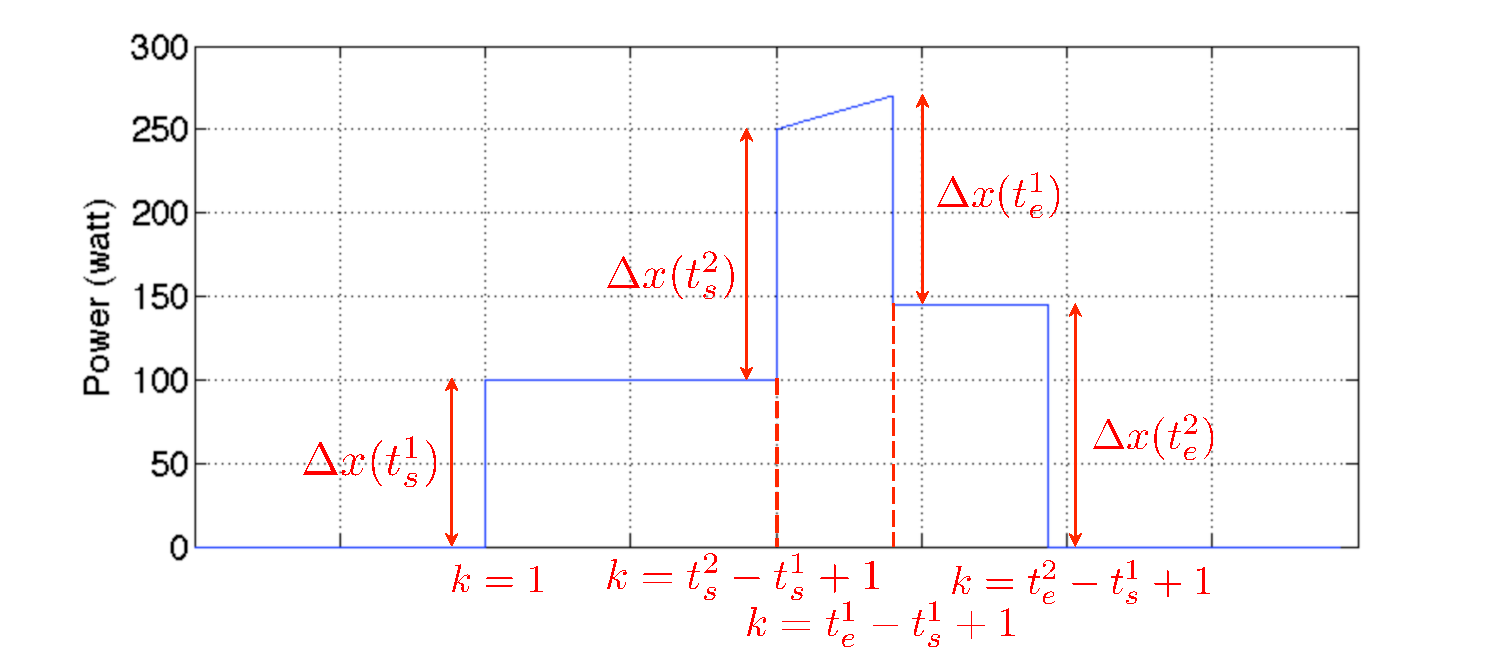
\includegraphics[width=0.8\textwidth]{./chapters/chapter4/images/dtwpattern.pdf}}
\caption{DTW pattern.}
\label{fig:dtw2}
%
\end{figure}
All possible patterns of each device are extracted and saved in library $\mathbf{DTWlib}$ from the training period. Because the length of patterns is different, the accumulated distance between the detected pattern $f^{dtw}$ and a pattern $j$ of device $i$ in the library is calculated by Algorithm~\ref{algo:DTW1}. Concretely,
\begin{equation}\label{eqDTW1}
\delta_{ij}^{dtw} = AccDistance(f^{dtw},f_{ij}^{dtw}).
\end{equation}
\begin{algorithm}
\caption{Accumulated distance between two different length vectors~\cite{Liao14}.} \label{algo:DTW1}
\begin{algorithmic}[1]
\Function{AccDistance}{$f1,f2$}
\State $l1 = \text{length}(f1)$
\State $l2 = \text{length}(f2)$
\State $\delta(0,0) = 0;\delta(i,0) = \delta(0,i) = +\infty$
	\For {$i=1,\ldots,l1$}
		 \For{$j=1,\ldots,l2$}
		    \State $d(i,j) = |f1(i)-f2(j)|$
		    \State $\delta(i,j) = d(i,j)+\min{\{\delta(i-1,j),\delta(i-1,j-1),\delta(i,j-1)\}}$
		 \EndFor
	\EndFor
	%\State \textbf{end for}
\State output = $\delta(l1,l2)$
\EndFunction
%\State \textbf{end function}
\end{algorithmic}
\end{algorithm}

In~\cite{Liao14}, the detected pattern will be matched to the device having a pattern with minimum accumulated distance calculated by Eq.~\eqref{eqDTW1}. 
However, in SmartSense, in order to improve the performance, the operating probability of each device during the same period as the detected event will also be used in log-linear form, and is defined as
\begin{eqnarray}
Pr_i^{dtw} &=& \prod_{t=t_s^1}^{t_e^{n_e}}{p_i(t)}\\
\phi_i^{dtw} &=& -\log{Pr_i^{dtw}}\nonumber \\
&=& -\sum_{t=t_s^1}^{t_e^{n_e}}{\log{p_i(t)}},\label{eqDTW2}
\end{eqnarray}
where $p_i(t)$ is the on-state probability of device $i$ at time instant $t$, estimated as in Section~\ref{model}, i.e. $p_i(t) =pr$ if device $i$ is detected as on and $p_i(t) = (1-npv)$ if detected as off. In the case of unsupervised devices, $p_i(t) = 0.5$. The load identification, as presented in Algorithm~\ref{algo:DTW2}, is not only based on the accumulated distance as in Eq.~\eqref{eqDTW1}, but also considers the operating probability of each device in Eq.~\eqref{eqDTW2}. The probability in log-linear form of all devices is contained in vector $\Phi^{dtw}$. A modified distance then combines these two parameters with a regularization parameter $\lambda_2$, which gives
\begin{equation}
d_{ij}^{dtw} = \delta_{ij}^{dtw} + \lambda_s\times \phi_i^{dtw}.
\end{equation}
The pattern giving the minimum distance will be selected to identify the corresponding device. Because the length of patterns strongly affects the accumulated distance, the DTW algorithm is only suitable for devices with fixed on-duration, such as fridge, washing machine, dish washer. Other devices controlled by the human intervention, e.g. lamp, computer, etc., cannot be exactly identified. Therefore, we propose to combine DTW with ED, in which $\mathbf{DTWlib}$ only contains the patterns of fixed on-duration devices and $\mathbf{EDlib}$ saves the edge patterns of the others. The flowchart of the proposed DTW algorithm is shown in Figure~\ref{fig:dtw1}. A threshold $\beta$ is used to reject a DTW pattern if it does not match with any one in $\mathbf{DTWlib}$. The detected pattern will be then extracted based only on the first rising edge and the last falling edge, by applying the ED procedure.
\begin{algorithm}
\caption{Matching detected event in DTW.}\label{algo:DTW2}
\begin{algorithmic}[1]
\Function{DTWiden}{$f^{dtw},\Phi^{dtw},\mathbf{DTWlib}$}
\State $MIN = +\infty$
\State $k = 0$
	\For {$i=1,\ldots,N$}
	    \State{$\phi_i^{dtw}=\Phi^{dtw}(i)$}
		 \For{$j=1,\ldots,m_i$}
		    \State $f_{ij}^{dtw} = \mathbf{DTWlib}\{i,j\}$
		    \State $\delta_{ij}^{dtw} = AccDistance(f^{dtw},f_{ij}^{dtw})$
		    \State $d_{ij}^{dtw} = \delta_{ij}^{dtw} + \lambda_2\times \phi_i^{dtw}$
		    \If{$d_{ij}^{dtw}\leq \beta$ and $d_{ij}^{dtw}\leq MIN$}
		        \State $MIN = d_{ij}^{dtw}$
		        \State $k = i$
		    \EndIf
		 \EndFor
	\EndFor
	%\State \textbf{end for}
\State output = $k$
\EndFunction
%\State \textbf{end function}
\end{algorithmic}
\end{algorithm}

\begin{figure}[!ht]
\centering
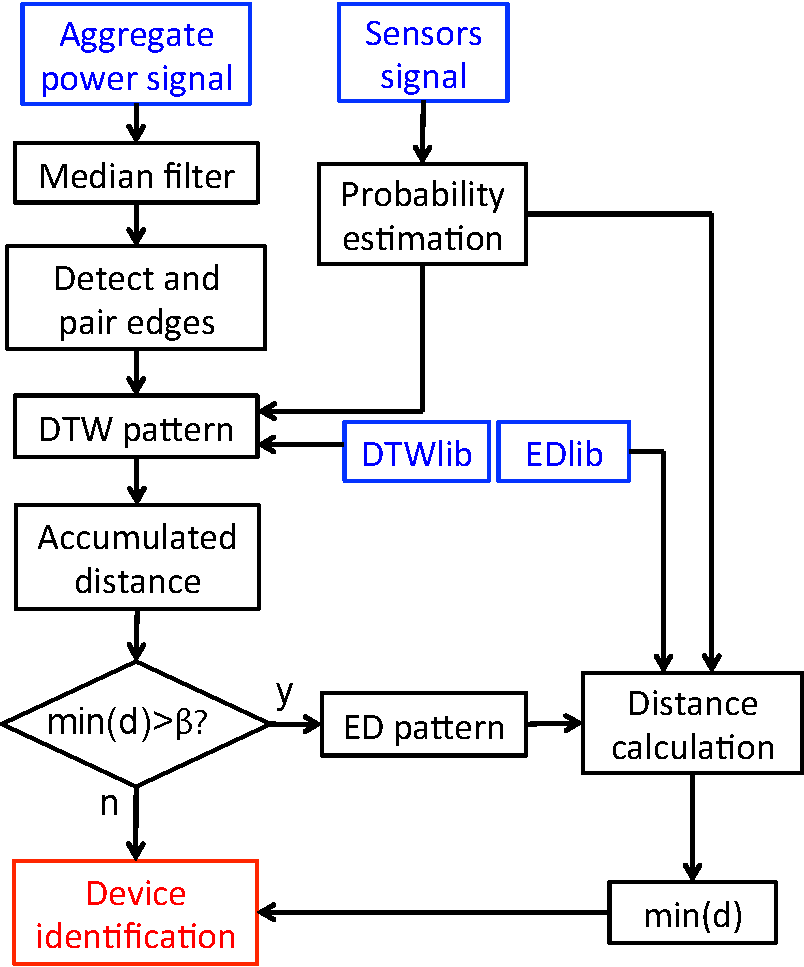
\includegraphics[width=0.65\textwidth]{./chapters/chapter4/images/DTWschema.pdf} 
\caption{Combination of DTW and ED algorithms. A threshold $\beta$ is used to reject a pattern if it does not match with any one in $\mathbf{DTWlib}$} 
\label{fig:dtw1} 
\end{figure}
